\section{Analysis techniques}
\label{sec:method}
%This section describes the estimator for measuring the angular power spectrum and the methodology for modeling it in the presence of PNG. We also demonstrate how we correct for the effects of survey geometry and integral constraint in the model power spectrum. Finally, we discuss how remaining systematic fluctuations are characterized using the cross-correlation between the LRG density and imaging properties and the mean density contrast of the LRG sample. 
 
 
\subsection{Power spectrum estimator}
For pixel $i$, the density contrast field $\delta_{i}$ is constructed from the observed density of galaxies $\rho_{i}$,
\begin{align}\label{eq:delta}
    \hat{\delta}_{i} &= \frac{\rho_{i}}{\hat{\overline{\rho}}} - 1,
\end{align}
and $\hat{\overline{\rho}}$ is the mean galaxy density estimated directly from the data,
\begin{equation}\label{eq:nbar}
\hat{\overline{\rho}} = \frac{\sum_{i}\rho_{i}f_{{\rm pix},i}}{\sum_{i}f_{{\rm pix},i}},
\end{equation}
where $f_{{\rm pix},i}$ represents the fractional area of pixel $i$, and is estimated by uniformly distributing random galaxies over the footprint. The angular power spectrum is then defined as the variance of the spherical harmonic transform of the field $\delta_{i}$,
\begin{equation}\label{eq:pusedocell}
        \hat{C}_{\ell} = \frac{1}{2\ell +1} \sum_{m=-\ell}^{\ell} |\hat{a}_{\ell m}|^{2},
\end{equation}
with,
\begin{equation}
        \hat{a}_{\ell m} = \frac{4\pi}{N_{{\rm pix}}} \sum_{i=1}^{N_{{\rm pix}}}  \hat{\delta}_{i}~f_{{\rm pix}, i}~ Y^{*}_{\ell m}(\theta_{i}, \phi_{i}),
\end{equation}
where $N_{\rm pix}$ is the number of non-empty pixels, and $\theta$ and $\phi$ represent the polar and azimuthal angular coordinates of the center for pixel \textit{i}, respectively. We the implementation of \texttt{anafast} from \citep[\textsc{HEALPix};][]{gorski2005healpix} to measure the angular power spectrum. The power spectrum estimator is biased because of the survey geometry; different harmonic modes are no longer independent and the measured power on scales near the survey size is zero. Later we will describe how we account for the effects in the model power spectrum, and validate the model against the lognormal simulations. 

 \subsection{Modeling}

 \begin{figure}
\centering
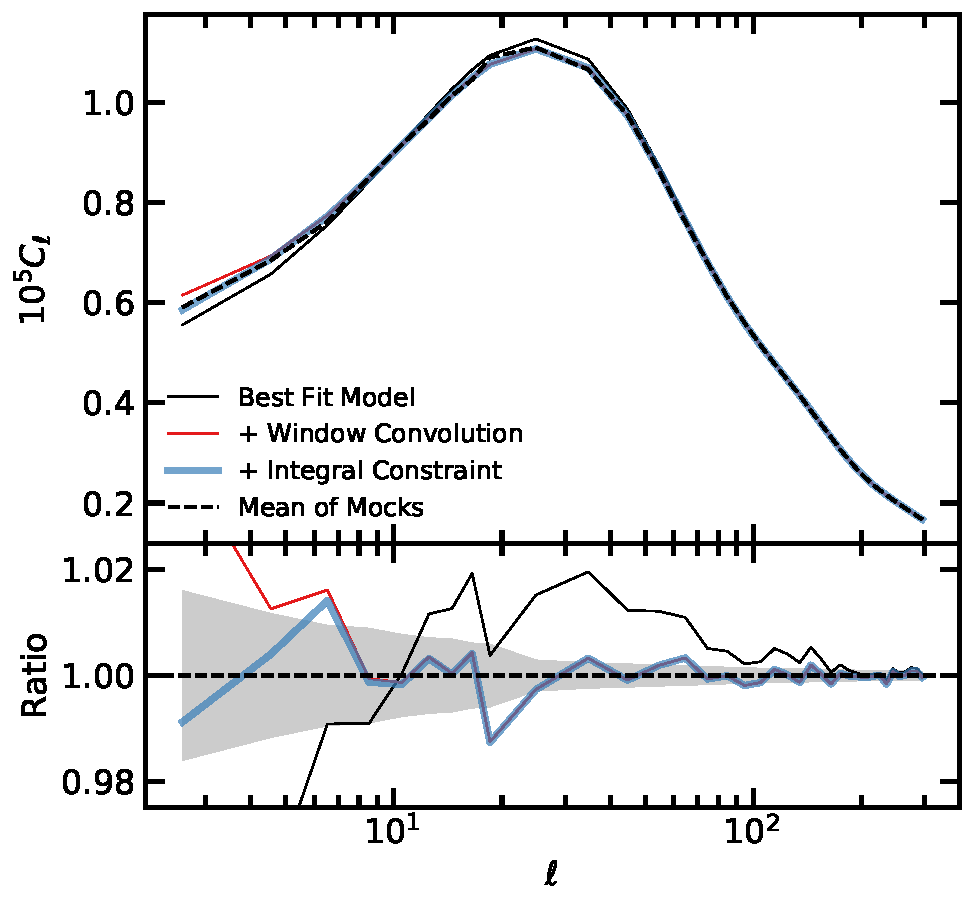
\includegraphics[width=0.5\textwidth]{model_mock.pdf}
\caption{Mean power spectrum of the lognormal density fields with $\fnl=0$ and best fit theoretical prediction after accounting for the survey geometry and integral constraint effects. Dark and light shades represent $1\sigma$ error on the mean and one realization, respectively. Bottom panel shows the residual power spectrum relative to the mean power spectrum of the mocks. No imaging systematic effects are added to these mocks.}\label{fig:model_mock}
\end{figure}

\subsubsection{Power spectrum}
The angular power spectrum is a projection of the 3D clustering of galaxies along the line of sight over all possible wavenumbers $k$. With redshift space distortions included, the projected angular power spectrum of galaxies is related to the 3D linear power spectrum $P(k)$ and shotnoise $N_{\rm shot}$ by \citep[see, e.g.,][]{Padmanabhan2007},
\begin{equation}\label{eq:cell}
    C_{\ell} = \frac{2}{\pi}\int_{0}^{\infty}\frac{dk}{k}k^{3}P(k)|\Delta_{\ell}(k)|^{2} + N_{\rm shot},
\end{equation}
where shotnoise is assumed to scale-independent, and kernel $\Delta_{\ell}(k) = \Delta^{\rm g}_{\ell}(k) + \Delta^{\rm RSD}_{\ell}(k)$ determines how much each wavenumber $k$ contributes to mode $\ell$ by integrating over all comoving scales $r$,
\begin{align}
    \Delta^{\rm g}_{\ell}(k) &= \int \frac{dr}{r} r b(r, k) D(r) \frac{dN}{dr} j_{\ell}(kr),\\
    \Delta^{\rm RSD}_{\ell}(k) &= - \int \frac{dr}{r} r f(r) D(r) \frac{dN}{dr} j^{\prime\prime}_{\ell}(kr),
\end{align}
where $D(r)$ is the normalized growth factor such that $D(0)=1$, $f(r)$ is the growth rate, and $dN/dr$ is the normalized redshift distribution of galaxies\footnote{$dN/dr = (dN/dz)*(dz/dr) \propto (dN/dz)*H(z)$} (see, Fig. \ref{fig:nz}). In the presence of local primordial non-Gaussianity, $b(r)$ is the linear bias $b$ (see, Fig. \ref{fig:nz}) plus the scale-dependent shift due to PNG (see, Eq. \ref{eq:db}),
\begin{equation}
b(k, r) = b + \frac{2 (b - p) \fnl \delta_{c}}{\alpha (k, r)},
\end{equation}
where $\alpha(k,r) \propto k^{2}D(r)$, $\delta_{c}=1.686$ is the critical density above which gravitational collapse occurs \citep{fillmore1984self}, and the parameter $p$ determines the response of the tracer to halo's gravitational field, e.g., $1$ for luminous red galaxies following universality and $1.6$ for tracers that are results of recent mergers like quasars. In order to overcome rapid oscillations in spherical Bessel functions, FFTLog\footnote{\href{https://github.com/xfangcosmo/FFTLog-and-beyond}{github.com/xfangcosmo/FFTLog-and-beyond}} algorithm and its extension as implemented in \cite{fang2020beyond} are employed to evaluate the inner integrations over $d\ln r$.

\subsubsection{Survey geometry and integral constraint}
For a galaxy survey that observes the sky partially, the measured power spectrum is convolved with the survey geometry. This means that the pseudo-power spectrum $\hat{C}_{\ell}$ obtained by the direct Spherical Harmonic Transforms of a partial sky map, differs from the full-sky angular spectrum $C_{\ell}$. However, their ensemble average is related by a mixing matrix \citep{hivon2002master}, 
\begin{equation}
    <\hat{C}_{\ell}> = \sum_{\ell^{\prime}} M_{\ell \ell^{\prime}}<C_{\ell^{\prime}}>,
\end{equation}
where $M_{\ell \ell^{\prime}}$ represents the mode-mode coupling from the partial sky coverage. This is known as the Window Function effect and a proper assessment of this effect is crucial for a robust measurement of the large-scale clustering of galaxies. This window effect is a source of observational systematic error and impacts the measured galaxy clustering, especially on scales comparable to survey size.

We follow a similar approach to that of \cite{chon2004fast} to model the window function effect on the theoretical power spectrum $C_{\ell}$ rather than correcting the measured pseudo-power spectrum from data. First, we use \textsc{healpix} to compute the pseudo-power spectrum of the window $\hat{C}^{\rm window}_{\ell}$, which is defined by a mask file in ring ordering format with \textsc{nside}$=256$. Then, we transform it to correlation function by,

\begin{equation}
    \omega^{\rm window} (\theta) = \frac{1}{4\pi}\sum_{\ell} (2\ell+1) \hat{C}^{\rm window}_{\ell} P_{\ell}(\cos \theta).
\end{equation}
Next, we normalize $\omega^{\rm window}$ such that it is normalized to one at $\theta=0$. Finally, we multiply the theory correlation function by $\omega^{\rm window}$ and transform the result back to $\ell$-space,%\footnote{We use Gauss-Legendre Quadrature to do the integration over $d\theta$.},
\begin{align}
    \hat{\omega}^{\rm model} &= \omega^{\rm model} \omega^{\rm window} \\
    \hat{C}^{\rm model}_{\ell} &= 2\pi \int d\theta \hat{\omega}^{\rm model}(\theta)P_{\ell}(\cos \theta).
\end{align}

By definition, the integral of the observed density contrast over the footprint vanishes,
\begin{align}\label{eq:ic}
    \sum_{i} \hat{\delta}_{i}~f_{{\rm pix},i} = 0,
\end{align}
and this boundary condition induces an effect in the measured power spectrum commonly referred to as the \textit{integral constraint}. We account for this effect in the modeling by,
\begin{equation}
     \hat{C}^{\rm model, IC}_{\ell} = \hat{C}^{\rm model}_{\ell} - \hat{C}^{\rm model}_{\ell=0} (\frac{\hat{C}^{\rm window}_{\ell}}{\hat{C}^{\rm window}_{\ell=0}})
\end{equation}

Fig. \ref{fig:model_mock} shows the mean measured power spectrum of 1000 lognormal density fields (dashed) and best fit theory prediction. light and dark shades represent the 68\% error on the mean and one single realization, respectively. DESI footprint mask is applied to the mocks, and even though DESI covers around $40\%$ of the sky, but the window effect is affecting modes down to $\ell=200$. On the other hand, integral constraint only alters the power in the first two bins.

\subsection{Parameter estimation}
Signature of local PNG is unique and cannot be reproduced with other cosmological parameters. We allow three parameters to vary; $\fnl$, shotnoise, and bias at $z=0$. Throughout this manuscript, we bin each mode with $\Delta\ell=2$ between $\ell=2$ and $20$ and $\Delta \ell=10$ from $\ell=20$ to $300$, while weighting each mode by $2\ell+1$. We also find that the distribution of power spectrum at the lowest bin, $2\leq \ell < 12$,  is not Gaussian and its standard deviation varies significantly from mocks with $\fnl=0$ to $76.9$ (see, Fig. \ref{fig:histcell}). Therefore, we attempt to fit $\log C_{\ell}$ to make our constraints insensitive to the choice of covariance matrix. The parameter $\fnl$ is constrained by maximizing a posterior defined as,
\begin{equation}
-2\ln\mathcal{L} = (\log C(\Theta)-\log \hat{C})^{\dagger} \mathbb{C}^{-1} (\log C(\Theta)-\log \hat{C}) + \chi^{2}_{\rm priors},
\end{equation}
where $\Theta$ represents the parameters, $\fnl$, bias at $z=0$, and shotnoise, all of which are associated with a flat prior, $\chi^{2}_{\rm priors}$; $C(\Theta)$ is the (binned) theoretical power spectrum including the effects for survey geometry and integral constraint; $\hat{C}$ is the (binned) measured power spectrum; and $\mathbb{C}$ is the covariance matrix constructed from simulations. 

\begin{figure}
\centering
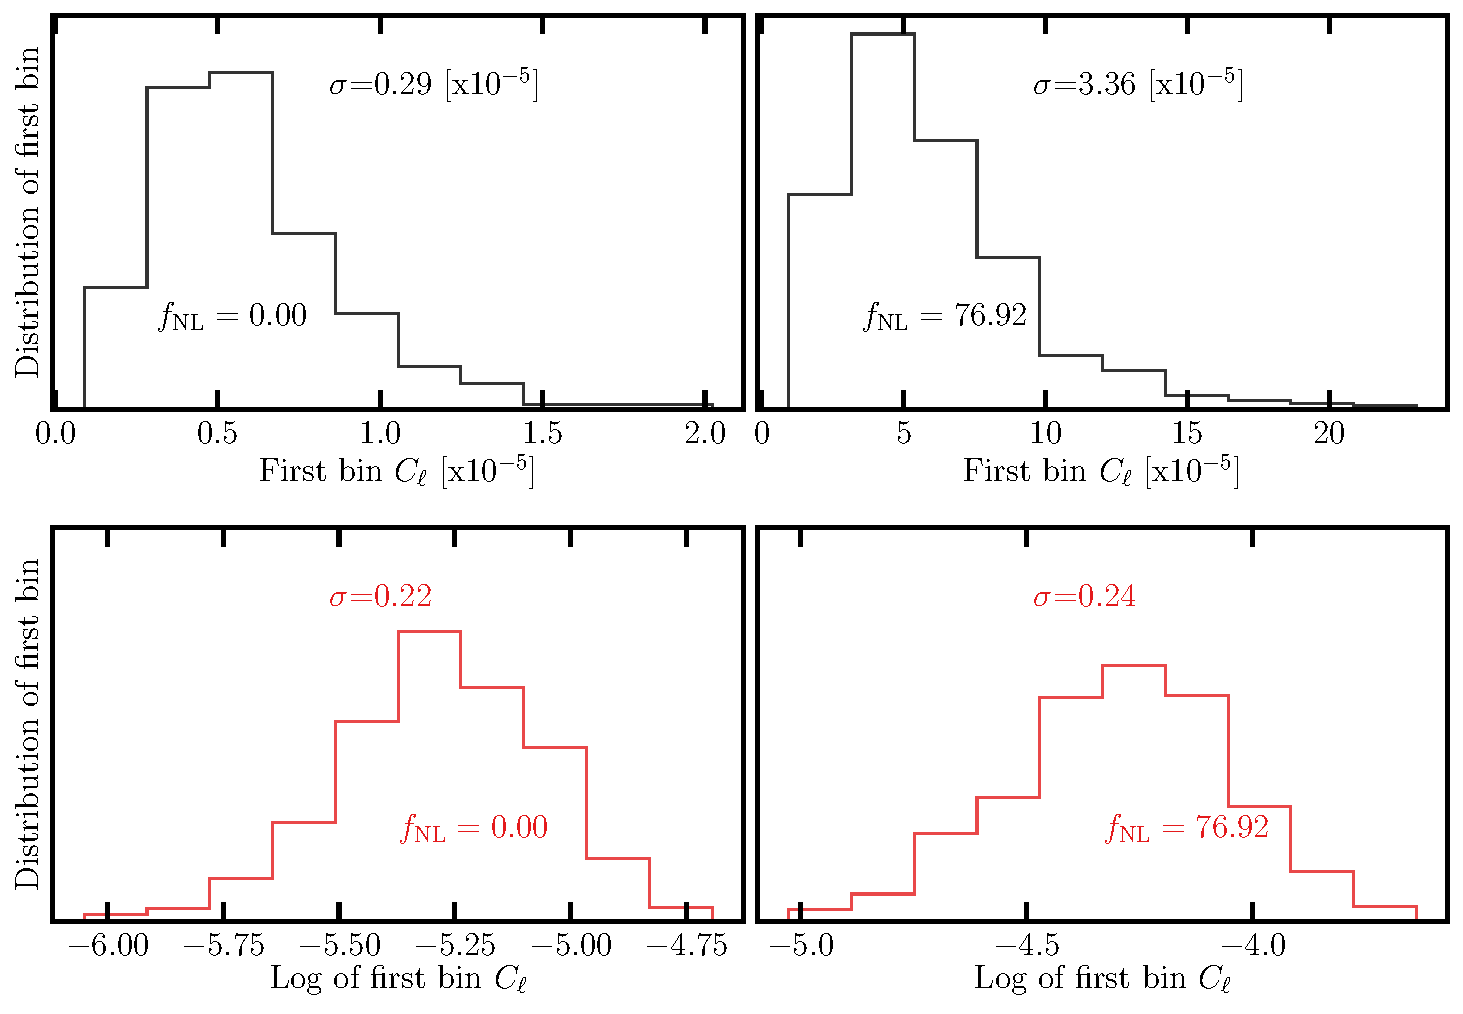
\includegraphics[width=0.5\textwidth]{hist_cl.pdf}
\caption{Distribution of the first bin power spectrum and its log transformation from the mocks with $\fnl=0$ (left) and $76.92$ (right). Differences in the standard deviations become less significant, and power spectrum measurements follow a more symmetric distribution after the log transformation.}\label{fig:histcell}
\end{figure}


\subsection{Remaining systematic errors}
\label{ssec:characterization}


We use the diagnostic tests first applied to SDSS data in \cite{rezaie2021primordial} based on cross power spectrum between galaxy density field and imaging maps and mean density contrast as a function of imaging properties to quantify the significance of imaging systematic effects. 

\begin{figure*}
\centering
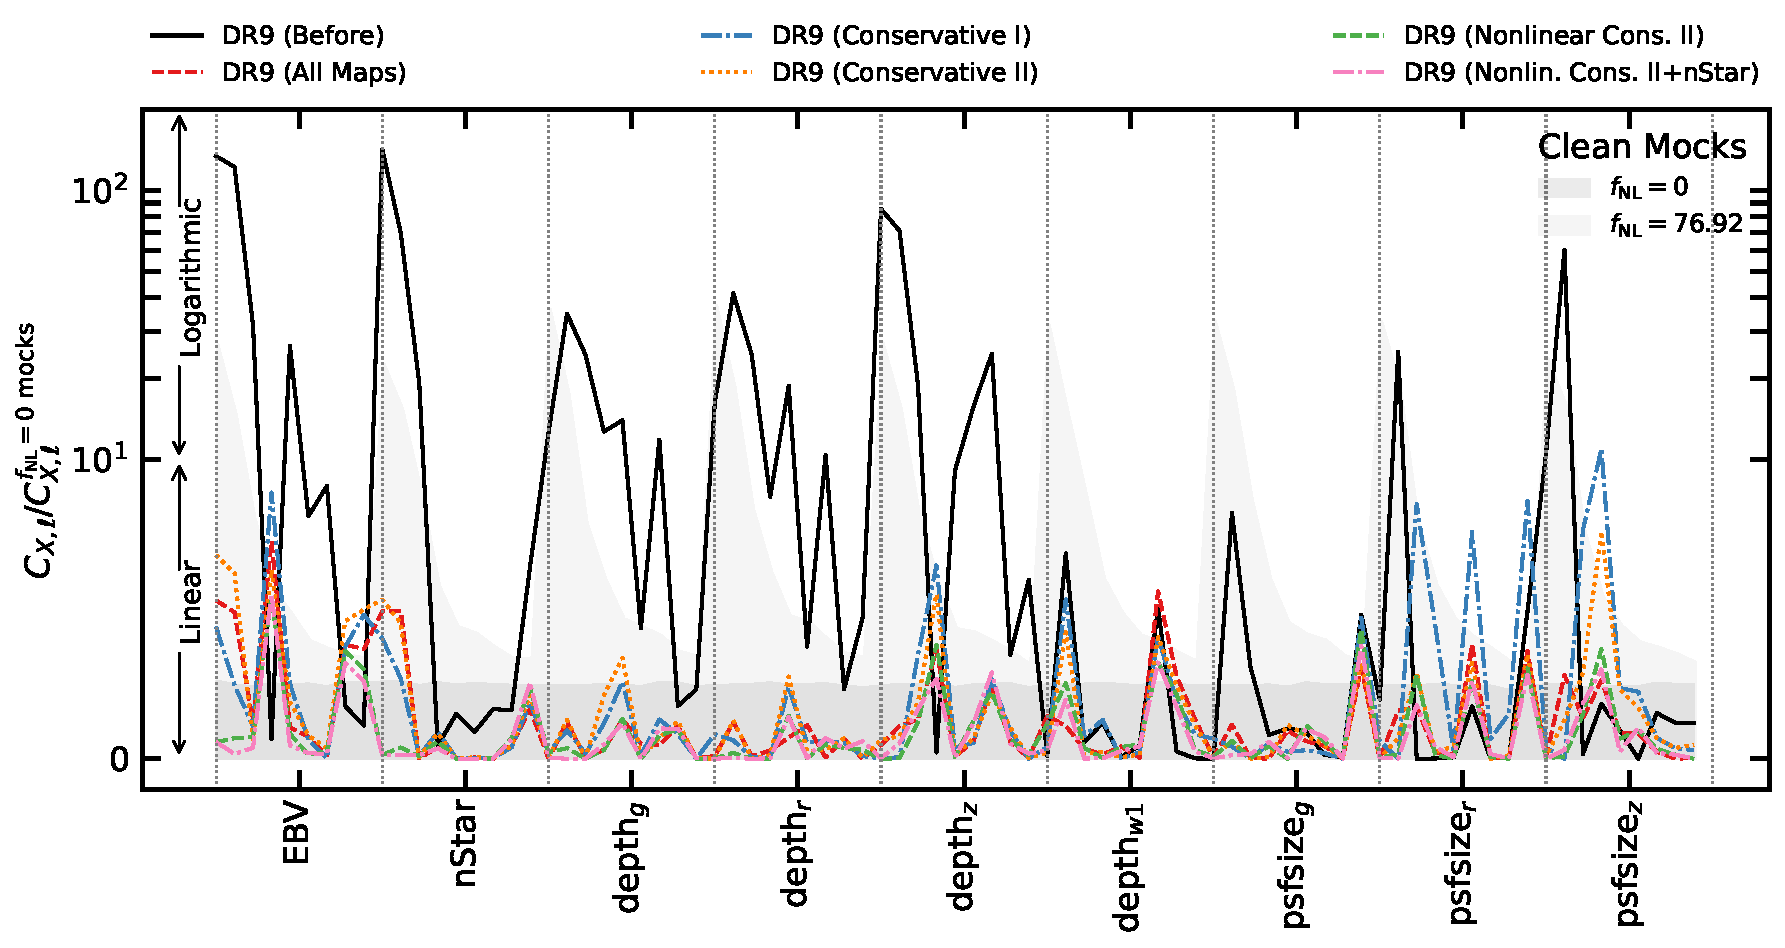
\includegraphics[width=0.76\textwidth]{clx_mocks.pdf}
\caption{Cross power spectra between the DR9 LRG sample and imaging maps. Dark and light shades represent the $97.5$ percentile of 1000 lognormal mocks without and with PNG, respectively.}\label{fig:clxmock}
\end{figure*}

\begin{figure*}
\centering
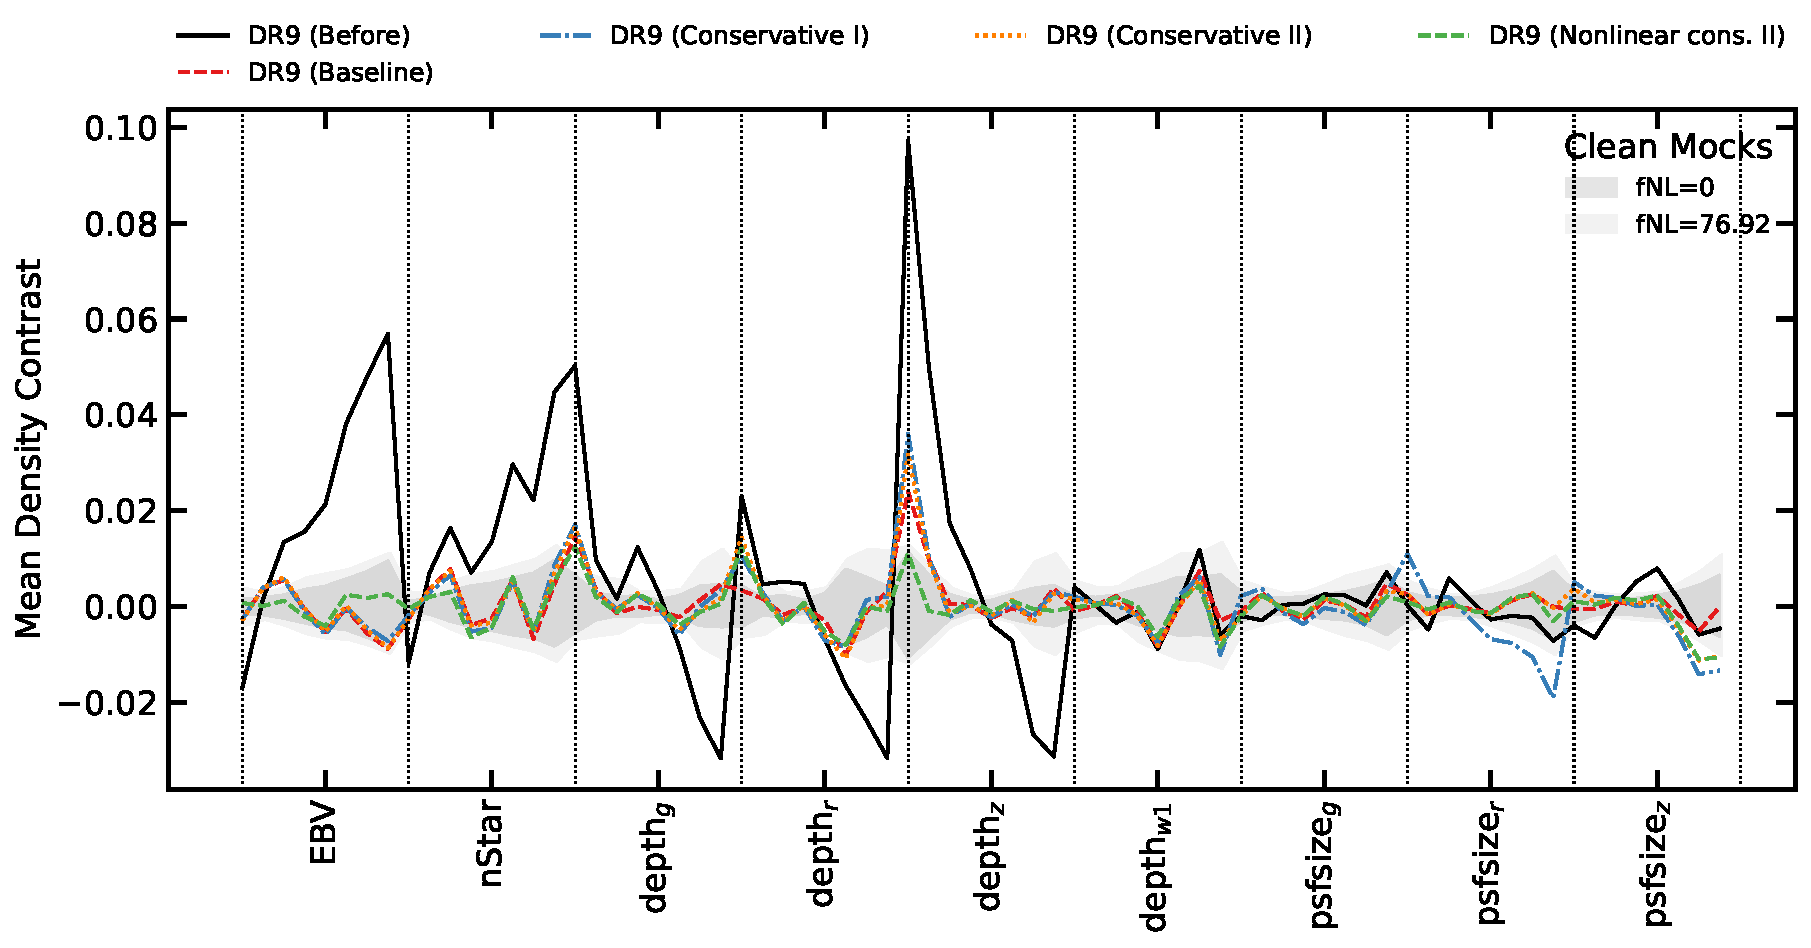
\includegraphics[width=0.76\textwidth]{nbar_mocks.pdf}
\caption{Mean density contrast of the DR9 LRG sample as a function of imaging maps. Dark and light shades represent the $1\sigma$ dispersion of 1000 lognormal mocks without and with PNG, respectively.}\label{fig:nbarmock}
\end{figure*}


\begin{figure}
\raggedleft
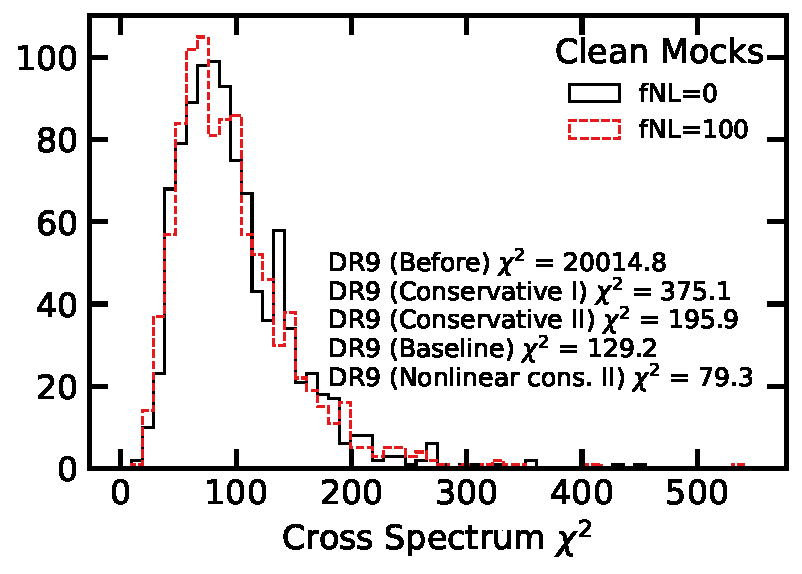
\includegraphics[width=0.45\textwidth]{chi2test.pdf}
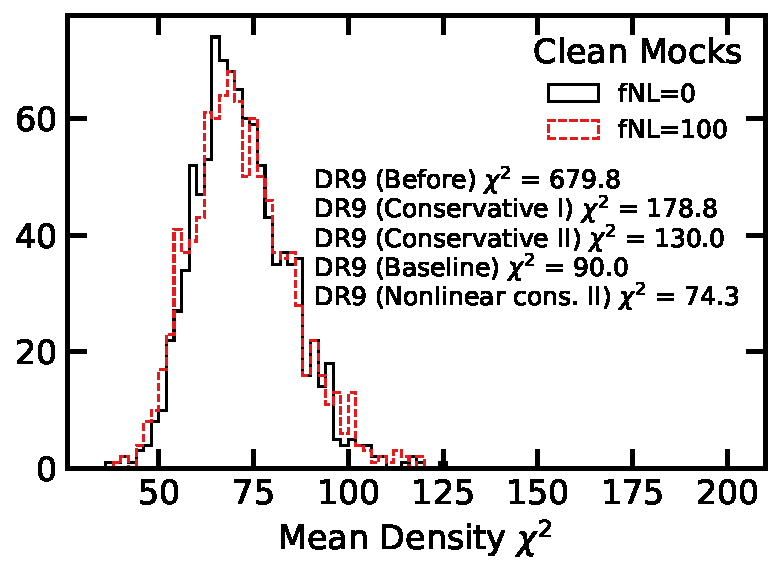
\includegraphics[width=0.44\textwidth]{chi2test2.pdf}
\caption{Remaining systematic error $\chi^{2}$ from the galaxy-imaging cross power spectrum (top) and the mean galaxy density contrast (bottom). The values observed in the DR9 sample before and after linear and nonlinear treatments are quoted, and the histograms are constructed from 1000 realizations of clean lognormal mocks with $\fnl=0$ and $76.92$.}\label{fig:chi2test}
\end{figure}

\begin{figure}
\centering
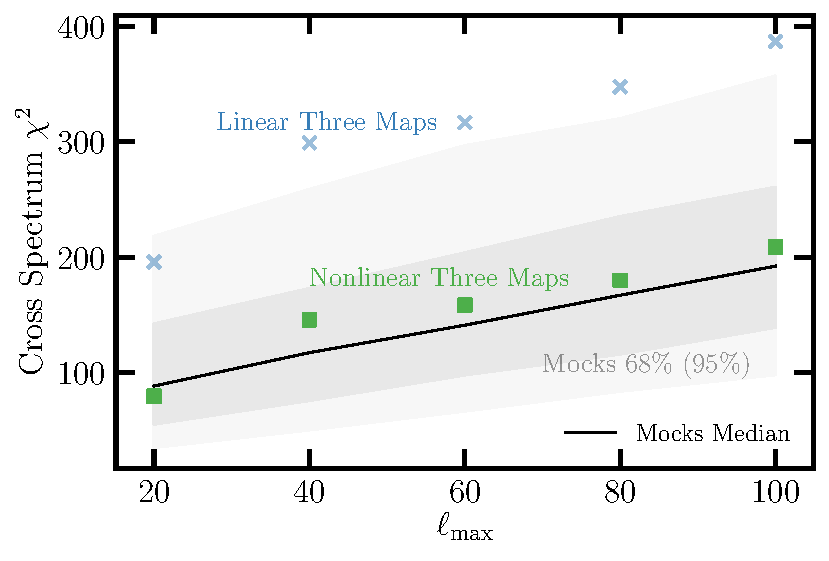
\includegraphics[width=0.5\textwidth]{chi2lmax.pdf}
\caption{Cross power spectrum $\chi^{2}$ as a function of the highest mode $\ell_{\rm max}$ for the DR9 LRG sample using the linear and nonlinear imaging weights with the conservative II maps. The lowest mode is fixed at $\ell_{\rm min}=2$. Solid curve and dark (light) shade represent the median estimate and $68\%$ ($95\%$) confidence constructed from the $\fnl=0$ mocks.}\label{fig:chi2cellextend}
\end{figure}


\subsubsection{Cross power spectrum}
Taking $C^{g,x}_{\ell}$ as the cross power spectrum between galaxy density contrast field and imaging map, one can normalize this quantity by auto power spectrum of imaging map itself:
\begin{equation}
\hat{C}_{x, \ell} = \frac{(\hat{C}^{g,x}_{\ell})^{2}}{\hat{C}^{x,x}_{\ell}},
\end{equation}
and then construct a vector from cross spectra against all other imaging maps:
\begin{equation}
\hat{C}_{X, \ell} = [\hat{C}_{x_{1}, \ell}, \hat{C}_{x_{2}, \ell}, \hat{C}_{x_{3}, \ell}, ..., \hat{C}_{x_{9}, \ell}].
\end{equation}
Finally, cross power spectrum $\chi^{2}$ can be defined as,
\begin{equation}
\chi^{2} = C^{T}_{X, \ell} \mathbb{C}_{X}^{-1} C_{X, \ell},
\end{equation}
where covariance matrix $\mathbb{C}_{X} = < C_{X, \ell} C_{X, \ell'} >$ is constructed from mocks without systematic effects. This statistics is measured for every mock realization with the leave-one-out technique to construct a histogram, which is then compared to the $\chi^{2}$ value observed from the DR9.  Fig. \ref{fig:clxmock} (top) shows the measured $C_{X}$ the DR9 sample before and after applying various imaging weights, relative to that of the mocks with $\fnl=0$. The dispersions of mocks with and without PNG are shown with the shade regions for comparison. We bin the $C_{X}$ measurements from $\ell=2$ to $20$ with $\Delta\ell=2$. The mean and standard deviation of $\hat{C}_{X, \ell}$ for 1000 mocks with and without $\fnl$ are shown in Fig. \ref{fig:clxmock}.  Extinction and stellar density have the highest cross power spectrum, and then depth in the z band. After applying the first version of weights with linear conservative I which includes extinction and depth-z, the cross power increases against psftsize in the r band. This indicates that only two maps are not sufficient to null out all of the cross correlations. With linear model there is residual power against extinction, depth-z, and psfsize-z; therefore, we apply weights based on a nonlinear model to account for more complex systematic effects. 

Fig. \ref{fig:chi2test} (top) shows the histogram of cross spectrum $\chi^{2}$ from mocks with and without $\fnl$. Comparing with the data, the residual is 20014.8 before correction, and after applying the first set of weights, it reduces to 375.1 with p-value \mr{XXX}. Adding psfsize-z, the linear model reduces the error dow to 195.9 (\mr{p-value = XXX}). Although using all maps gives the lowest error i.e., 129.2, but it could potentially lead to over-fitting true clustering given how correlated the imaging maps are (see, Fig. \ref{fig:pcc}). On the other hand, the nonlinear method with three maps yields a $\chi^{2}$ value of 79.3 and p-value of XXX, and adding the stellar density map reduces the error to 70.9 (p-value=XXX). This test clearly shows that a nonlinear approach is desired to get a null test. We further test the stability of our results by extending the highest mode from $\ell=20$ to $100$, or fluctuations over scales as small as $1.8$ degrees (see, Fig. \ref{fig:chi2cellextend}). The solid line shows how the median of 1000 mocks changes as the highest $\ell$ increases from $20$ to $100$. The red circles show the chi2 for the linear approach with three maps and the blue crosses show the chi2 for the nonlinear approach with three maps.

\subsubsection{Mean density contrast}
In the absence of systematic error, the integral of mean density contrast over the footprint should be zero As an alternative test, we calculate the histogram of the density contrast field relative to each imaging map.
\begin{equation}
\delta_{x} = ({\hat{\overline{\rho}}})^{-1} \frac{\sum_{i} \rho_{i} f_{{\rm pix}, i}}{\sum_{i} f_{{\rm pix}, i}},
\end{equation}
where the summations are over pixels in each bin of imaging map $x$. Similarly, we construct the mean density contract vector against all imaging maps,
\begin{equation}
\delta_{X} = [\delta_{x_{1}}, \delta_{x_{2}}, \delta_{x_{3}}, ..., \delta_{x_{9}}],
\end{equation}
and the total residual error as,
\begin{equation}
\chi^{2} = \delta_{X}^{T} \mathbb{C_{\delta}}^{-1} \delta_{X},
\end{equation}
where the covariance matrix $\mathbb{C}_{\delta} = < \delta_{X} \delta_{X}>$ is constructed from mocks without systematic effects. Fig. \ref{fig:clxmock} (bottom) shows the mean density contrast for the DR9 LRG sample. The shades represent the $1\sigma$ level fluctuations observed in 1000 clean mocks with $\fnl=0$ and $76.92$. Before treatment (solid) shows strong correlation around $10\%$ against depth in the z band which is consistent with the cross power spectrum. Beside that, there are strong positive trends against extinction and stellar density at about $5-6\%$. The linear model is able to mitigate most of the systematic effects with only the extinction and depth-z maps as input, however a new trend appears against psfsize-r which is indicative of psfsize dependence in the sample. This finding is in agreement with the cross power spectrum. Even after applying the linear weights there is some residual against depth-z at around $2\%$, which indicates the systematic effects might be more complex than what can be removed using a linear model. Nonlinear model with three maps (or four maps including the stellar density) is capable of reducing the fluctuations below $2\%$. 


Fig. \ref{fig:chi2test} (bottom) shows the mean density $\chi^{2}$ observed in the mocks vs DR9 sample before and after applying imaging weights. Linear weights with two maps reduce the chi-2 value from 679.8 (before) to 178.8. The p-value is indicative of remaining systematic effects. Adding psfsize-r does not help much with the p-value even though it reduces the chi-2 to 130. Using all maps with the linear model gives a more reasonable value however it leaves the analysis susceptible to over-fitting true clustering signal. With nonlinear approach two maps as input, the chi-2 is reasonable 74.3 with p-value XXX, and adding the stellar map does not change the p-value much, indicating the trend against stellar density can be explained with the extinction to a great extend. 